\documentclass[a4paper,11pt]{article}
\usepackage[francais]{babel}
%% Prévu pour compiler avec lualatex
% \usepackage[utf8]{inputenc}
\usepackage{fontspec}
\usepackage{libertine}
% \usepackage[T1]{fontenc}
\usepackage{graphicx}
\usepackage{fancyhdr}
\usepackage[top=2.5cm, bottom=2.5cm, left=2cm, right=2cm]{geometry}
\usepackage{listings}
\usepackage[utf8]{luainputenc}
\usepackage[hidelinks]{hyperref}
\usepackage{caption}

\lfoot{\bsc{Enseirb-Matmeca}}
\rfoot{Informatique --- 3\ieme{} année}

\pagestyle{fancy}
\begin{document}

\begin{titlepage}
  \begin{center}

    \begin{center}
      
\includegraphics[width=4cm]{EM.jpg}
    \end{center}

    \vspace*{1cm}
        
    \rule{0.75\linewidth}{0.7mm}\\[0.4cm]
    {\Huge Rapport TP1 --- PVM\\[0.4cm]}
    \rule{0.75\linewidth}{0.7mm} \\[1.5cm]

    {\Large Bazire Houssin\\Sylvain Vaglica\\Stéphane \bsc{Castelli}\\[2cm]}
    {\Large Mardi 29 Octobre 2013}
  \end{center}
\end{titlepage}

\tableofcontents
\clearpage
\section{Introduction}

PVM est une bibliothèque C et Fortran permettant la communication entre des processus sur une machine parallèle ou un cluster de machines ; elle utilise pour cela un démon lancé sur chaque machine qui se charge du routage des messages, du contrôle des processus et des problèmes pouvant survenir.Créée en 1989, PVM a au fil des décennies perdu en popularité au profit de MPI, mais reste un moyen efficace d'apporter une solution à des problèmes dont la résolution en séquentiel mettrait trop de temps. Au travers de ce projet, il a été réalisé un système distribué de craquage de mot de passe en force brute, sur le modèle maître / esclaves, avec un processus maître créant et distribuant des tâches, et des processus esclaves les exécutant. Un des objectifs principaux du projet, en plus de nous initier à la communication inter-processus et plus particulièrement à PVM, est d'analyser et optimiser la création et la répartition des tâches afin d'obtenir les meilleures performances possibles. Il sera d'abord explicité les choix qui ont été effectués, puis ils seront analysés.

\section{Réprésentation des données}
L'ensemble des mots de passe possibles de longueur maximale $p$ est un ensemble fini d'éléments énumérables  de la manière suivante:
\begin{itemise}
\item a, b, c, ..., o,
\item aa, ab, ac, ... ao, ba, bb, ... bo, .... oa, ob, ... oo,
\item .
\item .
\item .
\item $w_{p}$, le mot de longueur $p$ ne contenant que des 'o'
\end{itemise}
Chacun est conterti en un entier correspondant à sa position dans l'énumation. Il est alors possible de revenir ensuite au mot initial grâce à la fonction inverse. Grâce à cette conversion en entier, il est plus facile d'énumérer l'ensemble des possibilités car il suffit d'incrémenter un compteur puis de le convertir en chaine de caractères. En effet il suffit d'extraire le reste de la division par 15 (nombre de possibilités par caractère), pour obtenir la première lettre. On soustrait ce reste à l'entier, puis on divise par 15. On effectuer une nouvelle division et on en déduit la lettre suivante du reste et ainsi de suite jusqu'à avoir déterminé toutes les lettres.
%partie sur le nombre de possibilités à rajouter ici par Stephane


\subsection{GMP}
Comme expliqué dans la section précédente, le nombre de mot de passe possibles est exponentiel en la taille maximale du mot de passe. Or la PVM ne permet l'envoi de grands entiers que jusqu'à ceux pouvant être stockés dans une variable de type  \texttf{unsigned long} (le type \texttf{unsigned long long} n'étant pas supporté par PVM), c'est à dire ayant pour valeur maximale $2^{32}$. Ainsi pour des mots de passe de longueur supérieure à 8, on dépasse déjà la limite de stockage des entiers ($15^{8}$ ~ $2^{32}$ ). 

Nous avons donc décidé d'utiliser une bibliothèque spécifique pour le stockage des grands entiers. Plus précisément, la "GNU Multiple Precision Arithmetic Library" (http://gmplib.org/) aussi abrégée en GMP qui permet de s'affranchir des limitations de PVM et même de la librairie standard C.
Ainsi tous les calculs sont effectués sur des variables de type \texttf{mpz_t}. Et pour les envois de données, la valeur des ces variables est extraite et écrite en base 15 dans un tableau. Ce dernier est ensuite envoyé via PVM, le processus destinataire reçoit un ensemble d'octets (dont le nombre a été communiqué précédement), qui retransformé en type \texttf{mpz_t} pour pouvoir effectuer les opérations.


\section{Le maître}
Il s'occupe de démarrer les processus esclaves et de leur assigner les tâches. Le processus maître commence par envoyer à chaque esclave le mot de passe en clair, puis transforme l'ensemble des mots de passe possibles en un intervalle d'entiers (fonction bijective décrite dans la partie précédente). Chaque fois qu'un esclave demande du travail, il lui assigne un sous intervalle de l'intervalle initial, en lui donnant le début de l'intervalle et un pas (nombres d'entiers à tester).
Une gestion dynamique du pas est essentielle pour équilibrer le travail des esclaves et garantir une exécution la plus rapide possible. En effet, il est essentiel que l'ensemble des esclaves terminent le plus proche possible les un des autres.

\section{Les esclaves}
Chacun reçoit quand il le demande, un intervalle d'entiers correspondant à un certain nombre de mot de passe possibles à tester.
En effet, pour chaque entier de l'intervalle, l'esclave le convertit en une chaine de caractère et le compare ensuite grâce à la fonction \texttt{strcmp()} , au mot de passe réel reçu en argument lors de la création des processus esclaves par le maître. Si le résultat est positif, l'esclave communique au maître que l'exécution doit terminer car le mot de passe a été trouvé. Sinon, il continue jusqu'à arriver à la fin de son intervalle. Il communique alors avec le processus maître pour recevoir un nouvel intervalle de travail.


\section{La répartition des tâches}
% choix des intervalles
% demande de travail des esclaves
% attribution


\section{Changements en version multi-threadée}

\section{Performances}
\begin{figure}[h!]
  \centering
  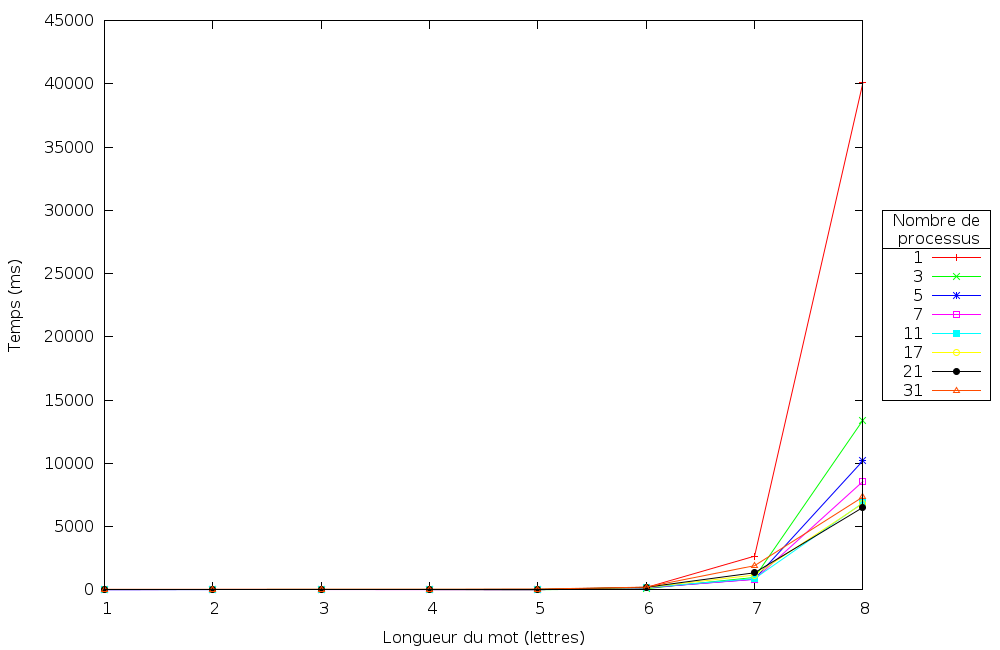
\includegraphics[width=\textwidth]{plot.png}
  \caption{Tests de performance}
  \label{perf}
\end{figure}
\section{Conclusion}




\end{document}
